%% This is file `elsarticle-template-1-num.tex',
%%
%% Copyright 2009 Elsevier Ltd
%%
%% This file is part of the 'Elsarticle Bundle'.
%% ---------------------------------------------
%%
%% It may be distributed under the conditions of the LaTeX Project Public
%% License, either version 1.2 of this license or (at your option) any
%% later version.  The latest version of this license is in
%%    http://www.latex-project.org/lppl.txt
%% and version 1.2 or later is part of all distributions of LaTeX
%% version 1999/12/01 or later.
%%
%% Template article for Elsevier's document class `elsarticle'
%% with numbered style bibliographic references
%%
%% $Id: elsarticle-template-1-num.tex 149 2009-10-08 05:01:15Z rishi $
%% $URL: http://lenova.river-valley.com/svn/elsbst/trunk/elsarticle-template-1-num.tex $
%%
\documentclass[preprint,12pt]{elsarticle}

\usepackage{isotope} % \isotope command

%% Use the option review to obtain double line spacing
%% \documentclass[preprint,review,12pt]{elsarticle}

%% Use the options 1p,twocolumn; 3p; 3p,twocolumn; 5p; or 5p,twocolumn
%% for a journal layout:
%% \documentclass[final,1p,times]{elsarticle}
%% \documentclass[final,1p,times,twocolumn]{elsarticle}
%% \documentclass[final,3p,times]{elsarticle}
%% \documentclass[final,3p,times,twocolumn]{elsarticle}
%% \documentclass[final,5p,times]{elsarticle}
%% \documentclass[final,5p,times,twocolumn]{elsarticle}

%% The graphicx package provides the includegraphics command.
\usepackage{graphicx}
%% The amssymb package provides various useful mathematical symbols
\usepackage{amssymb}
%% The amsthm package provides extended theorem environments
%% \usepackage{amsthm}

%% The lineno packages adds line numbers. Start line numbering with
%% \begin{linenumbers}, end it with \end{linenumbers}. Or switch it on
%% for the whole article with \linenumbers after \end{frontmatter}.
\usepackage{lineno}

%% natbib.sty is loaded by default. However, natbib options can be
%% provided with \biboptions{...} command. Following options are
%% valid:

%%   round  -  round parentheses are used (default)
%%   square -  square brackets are used   [option]
%%   curly  -  curly braces are used      {option}
%%   angle  -  angle brackets are used    <option>
%%   semicolon  -  multiple citations separated by semi-colon
%%   colon  - same as semicolon, an earlier confusion
%%   comma  -  separated by comma
%%   numbers-  selects numerical citations
%%   super  -  numerical citations as superscripts
%%   sort   -  sorts multiple citations according to order in ref. list
%%   sort&compress   -  like sort, but also compresses numerical citations
%%   compress - compresses without sorting
%%
%% \biboptions{comma,round}

% \biboptions{}

\journal{Journal Name}

\begin{document}

\begin{frontmatter}

%% Title, authors and addresses

\title{Adding Precision Time Structure to Neutrino Beams for Energy and Flavor Discrimination}

%% use the tnoteref command within \title for footnotes;
%% use the tnotetext command for the associated footnote;
%% use the fnref command within \author or \address for footnotes;
%% use the fntext command for the associated footnote;
%% use the corref command within \author for corresponding author footnotes;
%% use the cortext command for the associated footnote;
%% use the ead command for the email address,
%% and the form \ead[url] for the home page:
%%
%% \title{Title\tnoteref{label1}}
%% \tnotetext[label1]{}
%% \author{Name\corref{cor1}\fnref{label2}}
%% \ead{email address}
%% \ead[url]{home page}
%% \fntext[label2]{}
%% \cortext[cor1]{}
%% \address{Address\fnref{label3}}
%% \fntext[label3]{}


%% use optional labels to link authors explicitly to addresses:
%% \author[label1,label2]{<author name>}
%% \address[label1]{<address>}
%% \address[label2]{<address>}

\author{Andrey Elagin[UofC], Jonathan Eisch[ISU], Henry Frisch[UofC], Sergei Nagaitsev[Fermilab,UofC], Matthew Wetstein[ISU]}
\address[UofC]{Enrico Fermi Institute, University of Chicago, Chicago IL 60637}
\address[Fermilab]{Fermi National Laboratory, Batavia IL 60510}
\address[ISU]{Matt to Fill in}

\begin{abstract}
%% Text of abstract
New advances in photodetector technology may enable the detailed resolution of energy and flavor substructure in neutrino beams. A number of notable analyses by the MINOS and MiniBooNE collaborations have  looked at detailed features in the arrival time of neutrino bunches. Pushing that capability to finer time scales would allow selecting different neutrino energy and flavor spectra based on the arrival time of the neutrinos relative to the parent proton bunch time. Later neutrinos correspond to slower, and therefore lower energy, parent hadrons. In addition the fractions of tau, muon, and electron neutrinos (antineutrinos) varies with the arrival time. We show that these effects could be resolved by detectors with order 100 psec vertex time resolution, but that the discrimination is limited by the current bunch size of the protons impinging on the target. Shortening the width of neutrino bunches to well below 500 psec would substantially enhance this effect. As opposed to off-axis experiments, which  can only sample a small slice of the angular flux spectrum, this `stroboscopic' approach is analogous to sampling multiple off-axis angles with on-axis detectors, and is applied equally to both near and far detectors in an oscillation experiment. 
\end{abstract}



\begin{keyword}
Timing \sep Timing, Neutrino \sep Neutrino, Oscillation \sep Oscillation, RF-Structure \sep RF-Structure, Proton Bunch \sep Proton Bunch
%% keywords here, in the form: keyword \sep keyword
%% MSC codes here, in the form: \MSC code \sep code
%% or \MSC[2008] code \sep code (2000 is the default)

\end{keyword}

\end{frontmatter}

%%
%% Start line numbering here if you want
%%
\linenumbers

%% main text
\section{Introduction}
\label{sec:intro}

The discovery of Charge-Parity (CP) violation in the neutrino sector hinges on high precision, increasingly systematics-dominated measurements of neutrino oscillation parameters. The dominant systematic uncertainties...

The wide span of energies in neutrino beams stems from the wide range of energies among the parent hadrons and is limited by the ability to cool and focus those beams. One handle for controlling and understanding the beam flux is to look at angles off-axis from the pointing of the beam, a technique notably exploited by the NOvA and T2K experiments.

Another handle for understanding and selecting different energy spectra within a neutrino beam exploits the differing velocities of the parent hadrons. Lower energy pions and kaons travel more slowly, especially as they approach sub-relativistic energies. As a consequence, lower energy neutrinos start further behind the rest of the bunch and selecting later arriving neutrinos would provide an increasingly pure low-energy subset of the overall flux.

The idea of using timing to resolve beam structure has a long history. Efforts to detect dark matter have relied on time-of-flight differences between dark matter particles and neutrinos. Timing has successfully been employed to identify a pure sample of stopped kaons and pions in neutrino beams. Several notable efforts have utilized bunch timing to place limits on neutrino velocity. MINOS, in particular, noted interesting kinematic relationships within the beam time. The MiniBooNE collaboration even explored the idea of using timing to select on the neutrino energy spectrum. However, efforts to select different energy spectra on the basis of beam timing have been largely overlooked due to two considerations: (1) Limited time resolutions of the detectors themselves were insufficient to see the O(100) psec effect, and (2) the $\sim$900 psec spread of the proton bunch impinging on the target washes out most of the effect.

In this paper, we revisit the idea of using beam timing to select different energy components of the neutrino flux. We show that existing precision timing technology is capable of resolving O(100) psec time-of-flight differences in neutrinos arrival times. {\it More importantly, we argue that feasible modifications to existing proton beams could superimpose a hyper-fine bunch structure on the protons, providing short enough bunches, spaced widely enough to fully exploit the energy spreading effect.}

The power of this technique stems from the fact that, in contrast to off-axis measurements, the different neutrino energy spectra can be selected within the same detector. Moreover, these timing relationships can be applied in near and far detector alike.

\begin{figure}[t]
	\begin{center}
           	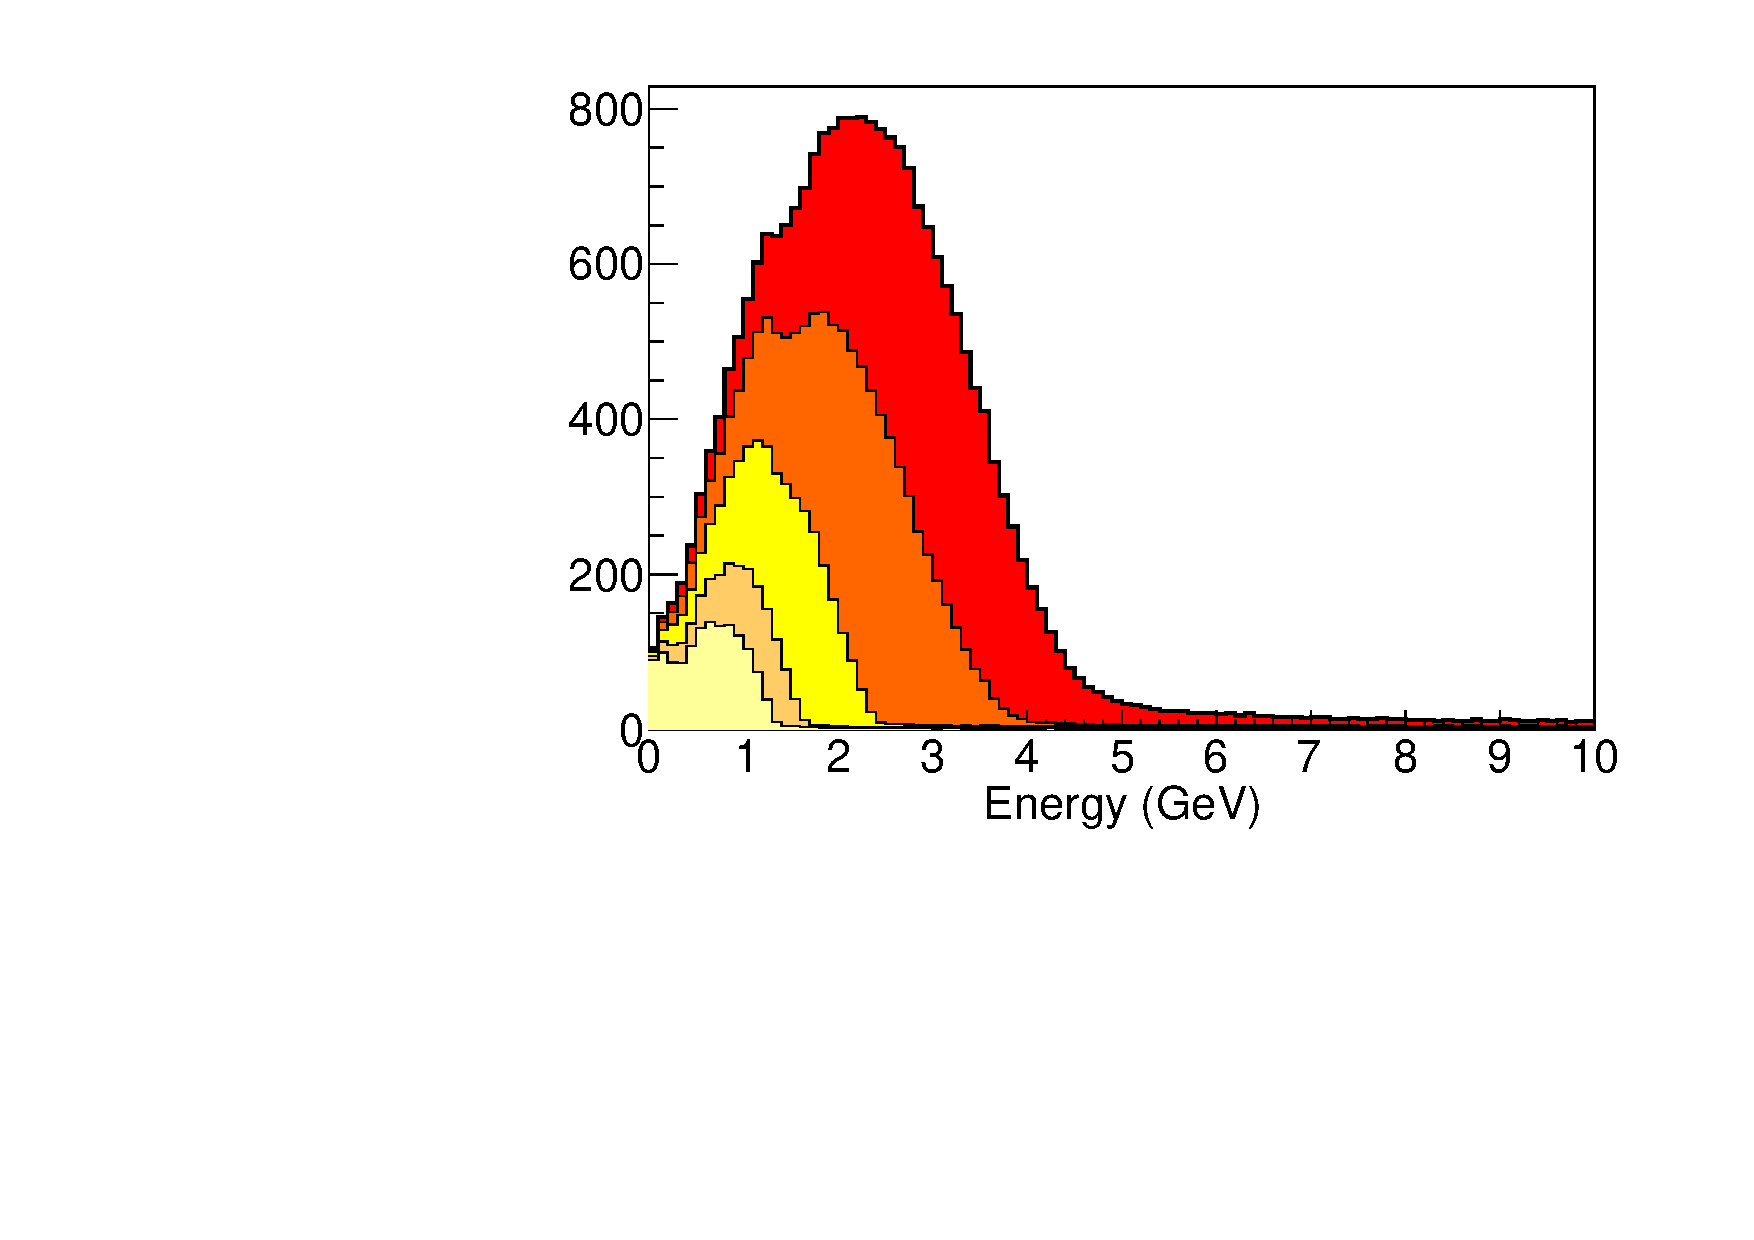
\includegraphics[width=1.0 \linewidth]{Figures/2018.10.10_LBNFtiming/DUNEbeam_truetimingB.pdf}
	\end{center}
	\caption{The DUNE forward horn current flux (red), with the fluxes corresponding to increasingly later time-cuts on the bunch time, assuming no time spread of the protons on target: 250 psec after the start of the neutrino bunch (orange), 500 psec after (yellow), 750 psec (dark beige), 1 nsec (light beige).}
		\label{fig:anniedetector}
\end{figure}


\begin{figure}[t]
	\begin{center}
           	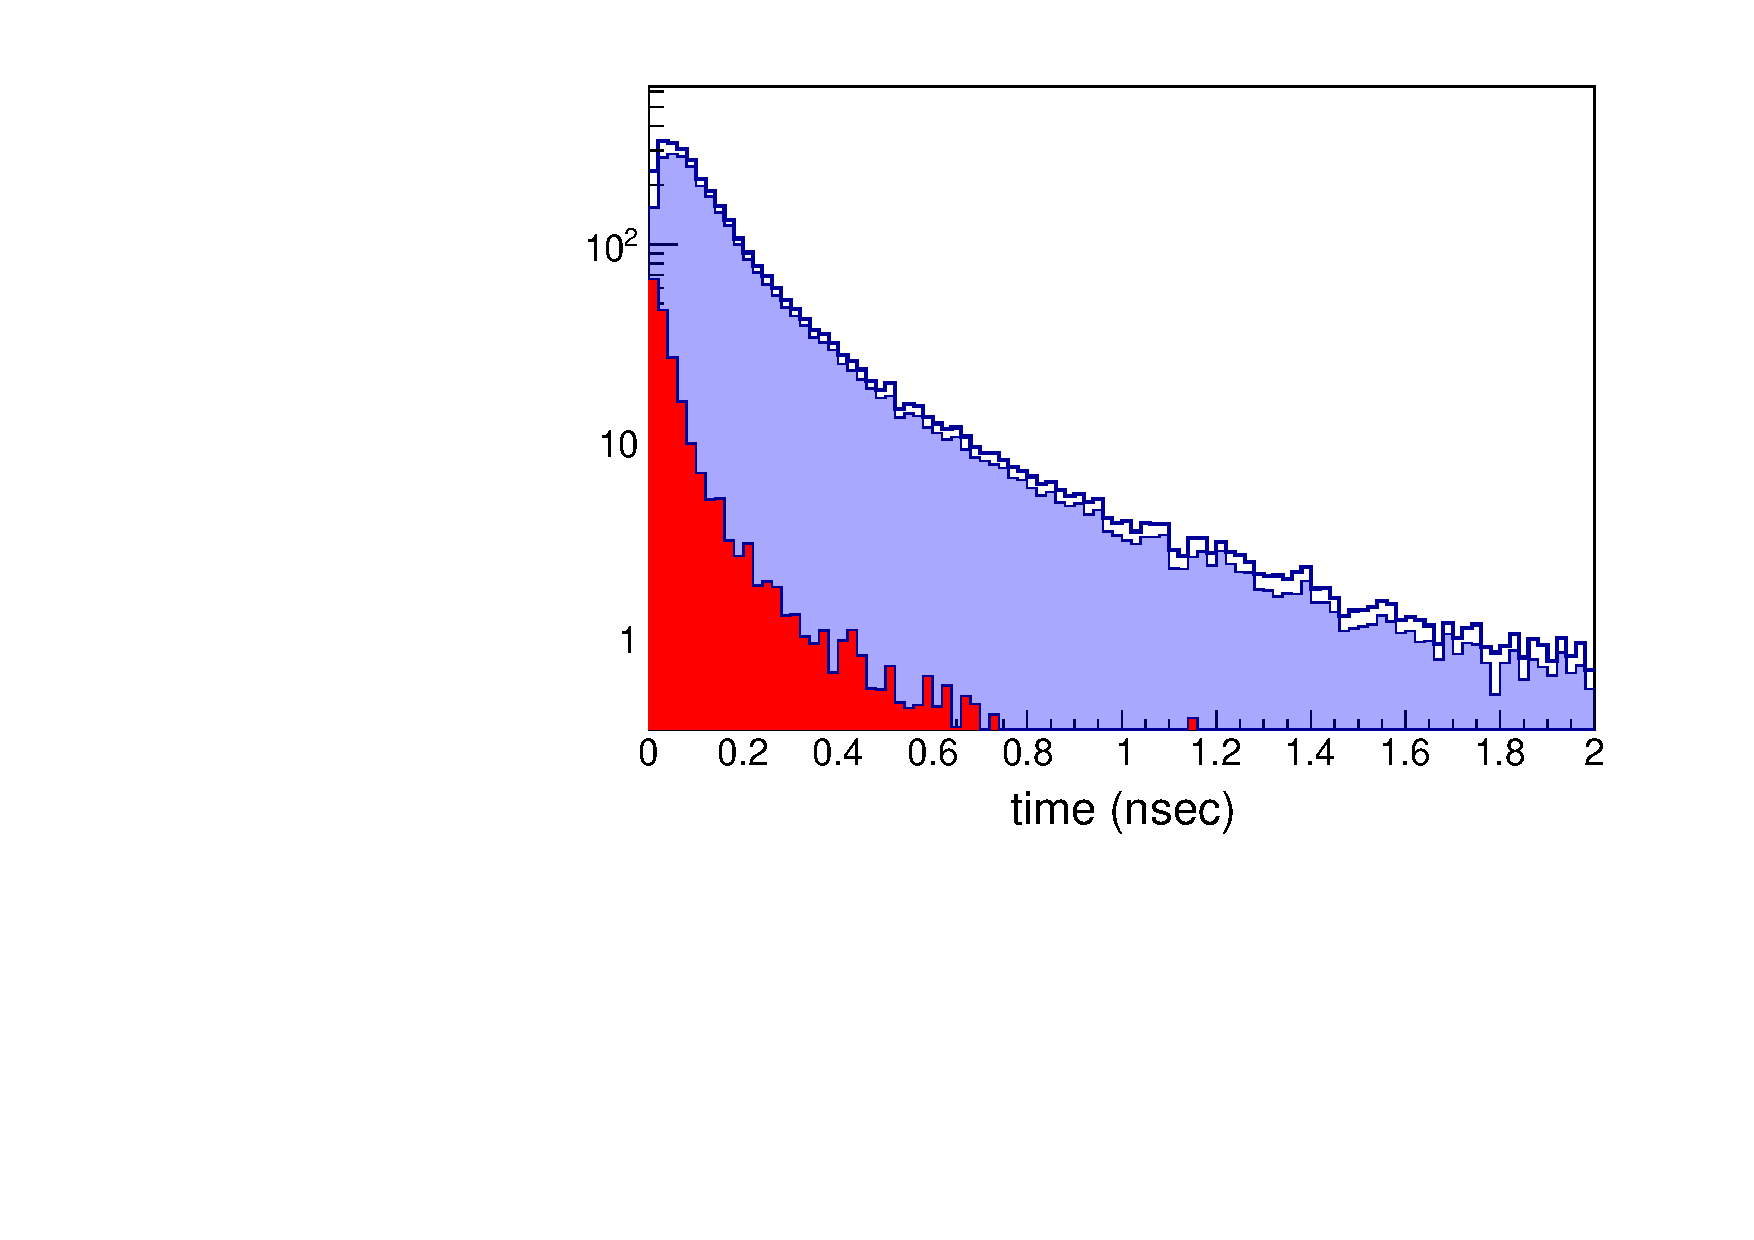
\includegraphics[width=0.8 \linewidth]{Figures/2018.11.07_LBNFtimingRHC/RHCbeamcontent_log.pdf}
	\end{center}
	\caption{The time spectrum of anti-neutrinos in reverse horn current mode (blue) overlaid with wrong-sign neutrino contamination in red. The wrong-sign component drops off more quickly.}
		\label{fig:anniedetector}
\end{figure}

\section{The Mechanism}

The difference in arrival time of a neutrino from a sub-relativistic pion of energy E' with respect to a high energy pion travelling with speed $\sim$c is given by:

\begin{equation}
\Delta t(E') = \frac{c - v(E')}{c} \tau (E')
\end{equation}

Where $\tau (E')$ is the lifetime of the lower energy pion in the lab frame. The time spreading will only occur until the decay of the lower energy pion, at which point the daughter neutrinos will propagate at c. The lifetime of the higher energy pion is irrelevant, since the pion is already propagating at roughly c.

\begin{equation}
\Delta t(E') = \tau (E') [1 - \beta (E')]
\end{equation}

\begin{equation}
\Delta t(E') = (\frac{E'}{m} \tau_0) [1 - \sqrt{ 1 - \frac{m^2}{E'^2}}]
\end{equation}

\begin{equation}
\Delta t(E') = [\frac{E'}{m} - [1 - \sqrt{ \frac{E'^2}{m^2} - 1}] \tau_0
\end{equation}

As one would expect, at the lowest energies, where the pion is essentially at rest in the lab frame, $\Delta t(E')$ approaches the lifetime of the pion in the rest frame, $\tau_0$. At high energies, the speed of the lower-energy pion approaches that of the higher energy pion and thus $\Delta t(E')$ goes to zero. 

\begin{figure}[t]
	\begin{center}
           	\begin{tabular}{c c}	
           	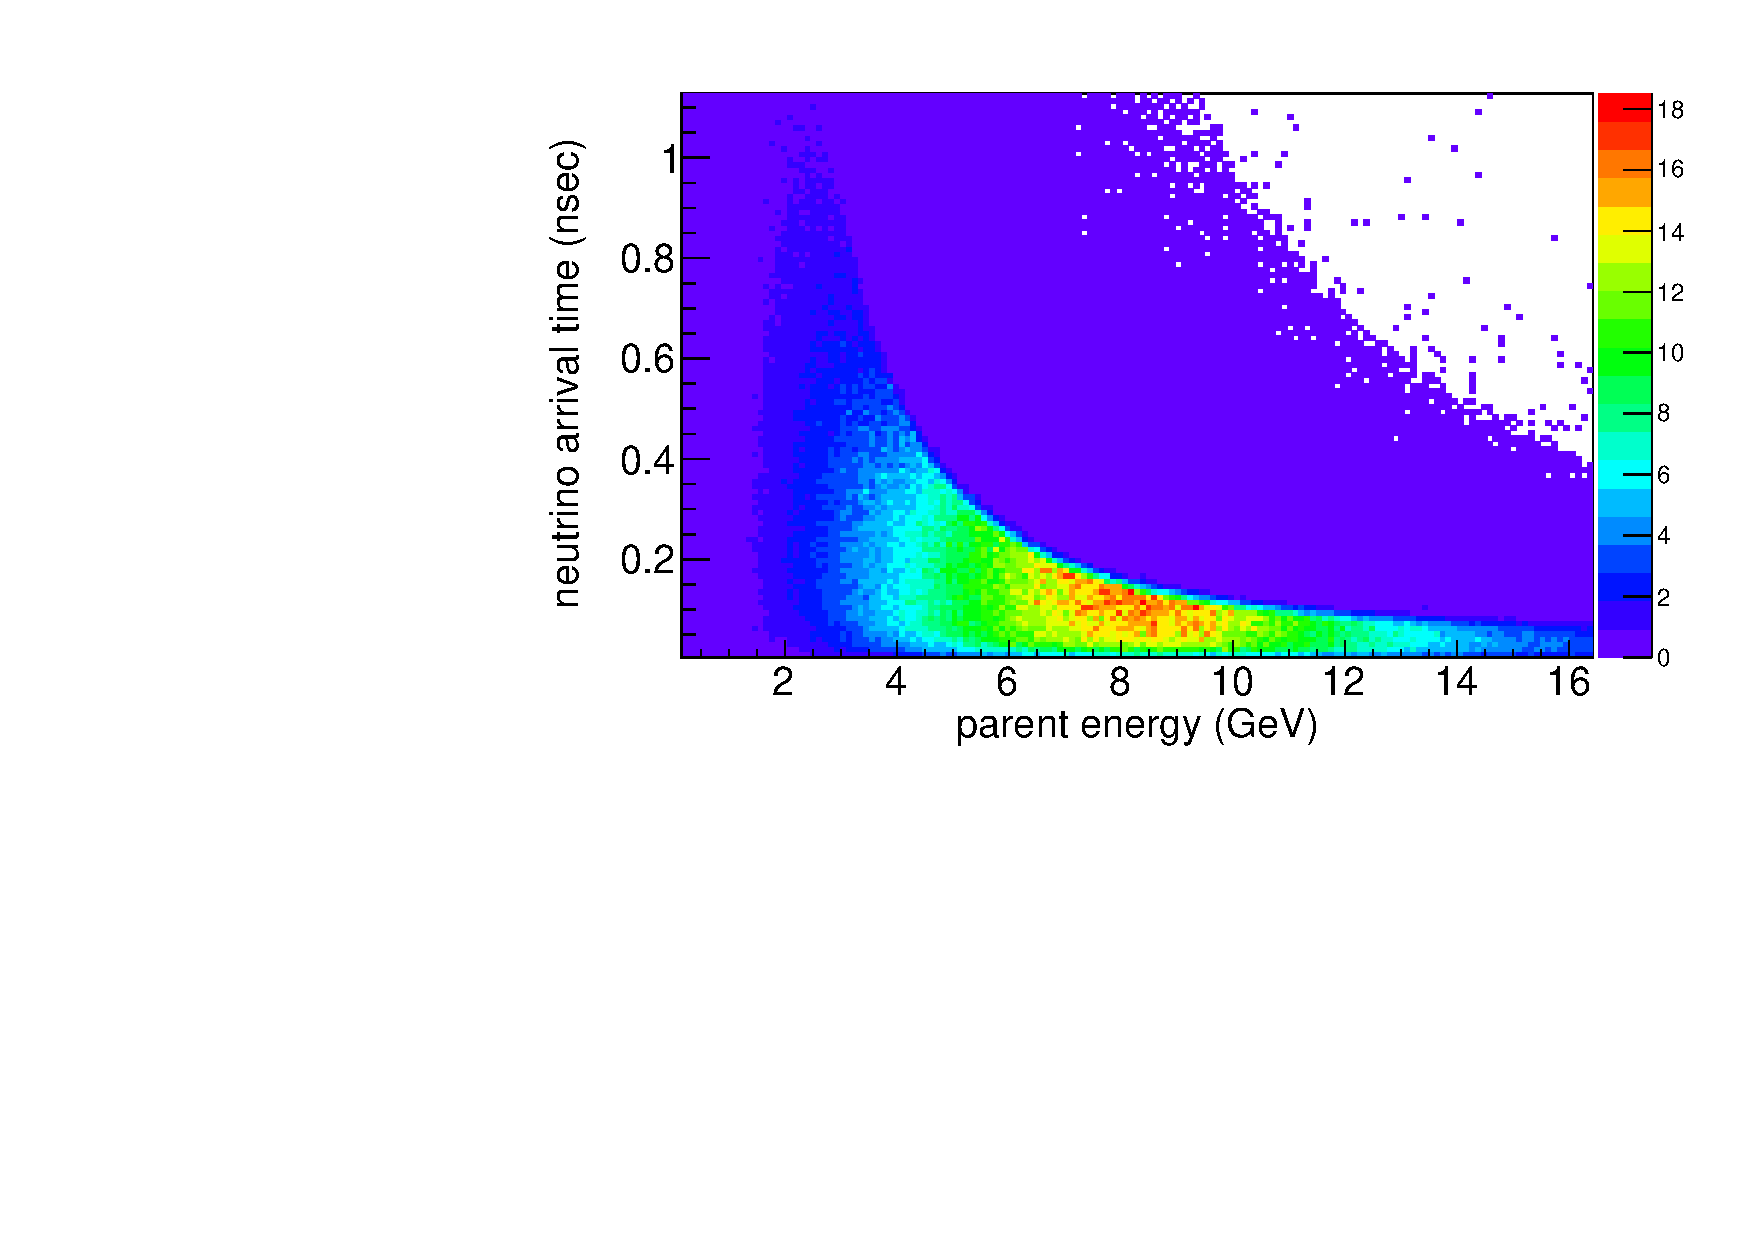
\includegraphics[width=0.49 \linewidth]{Figures/2018.10.14_LBNFtiming/parentEvsdT.pdf} &
			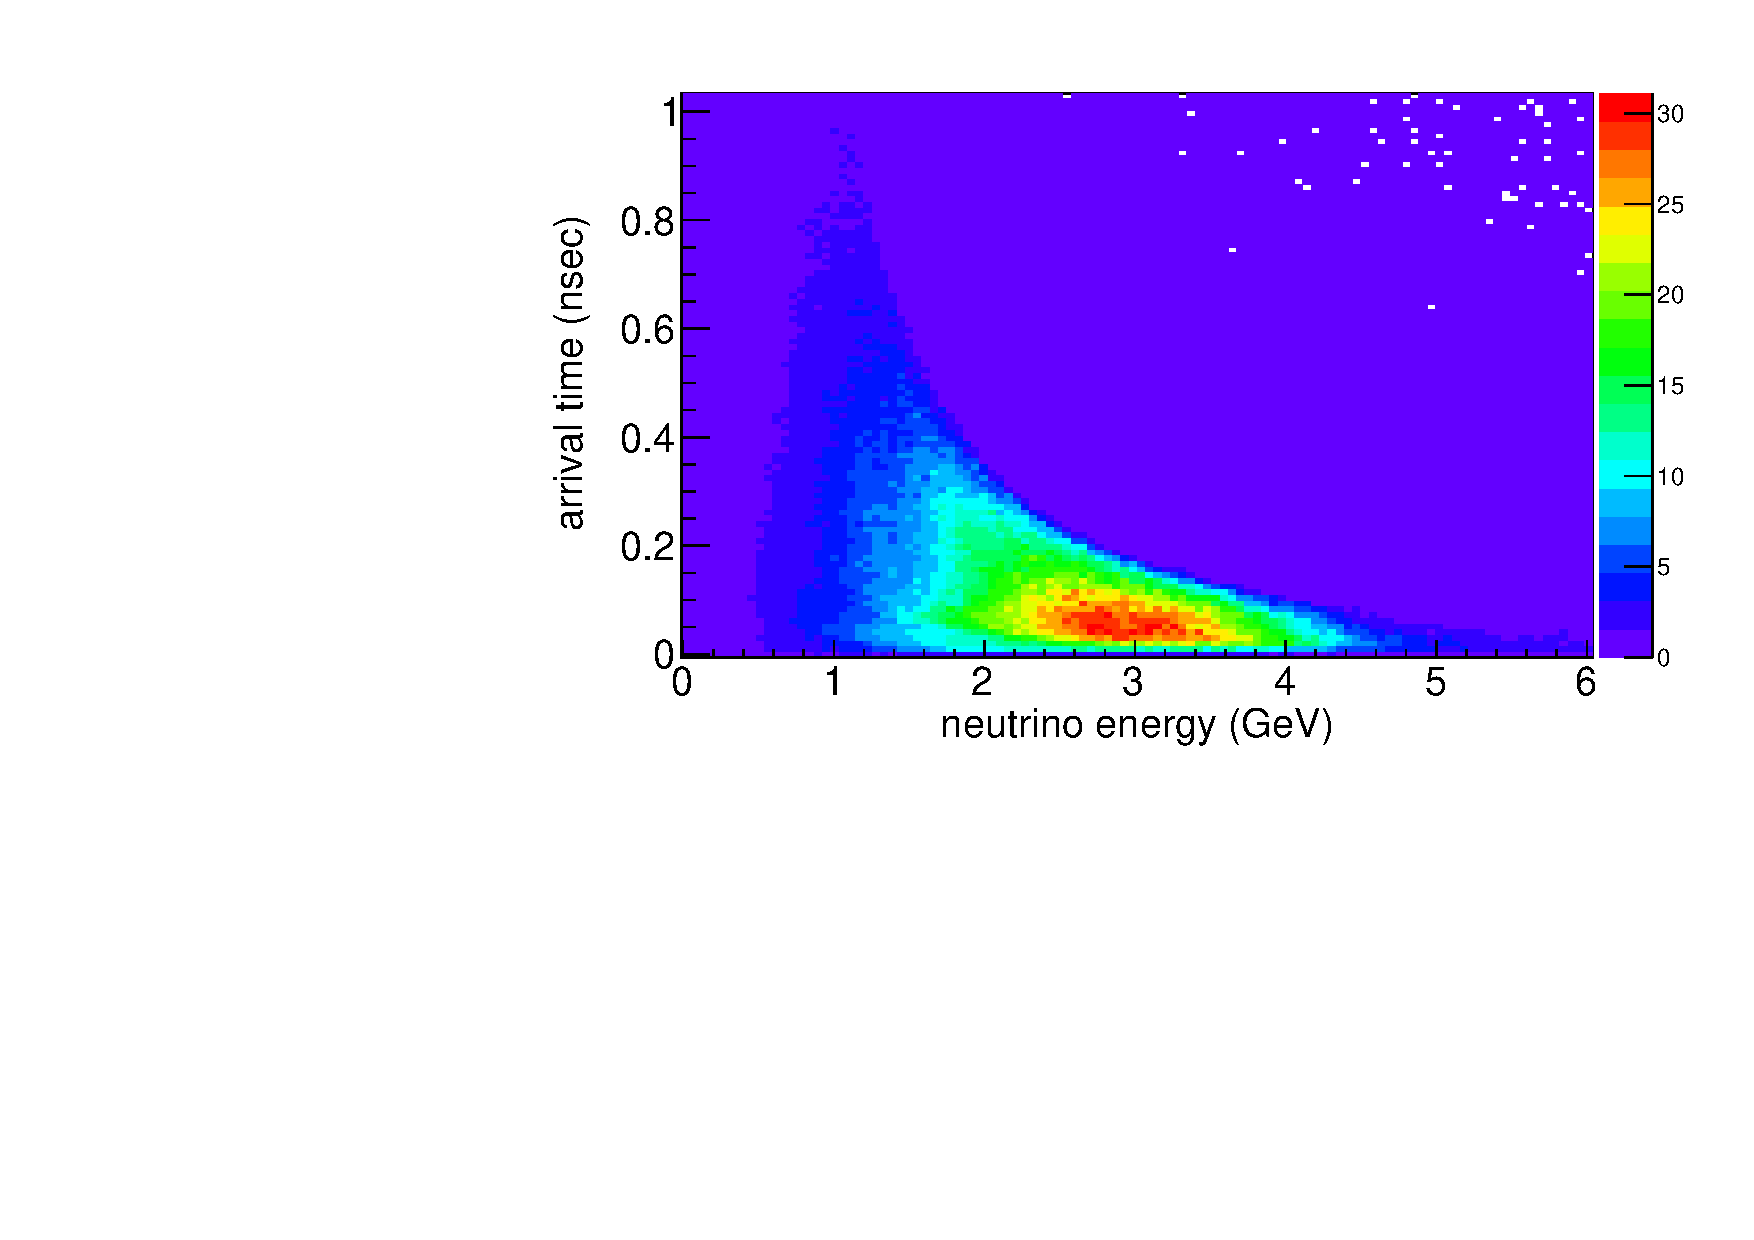
\includegraphics[width=0.49 \linewidth]{Figures/2018.10.14_LBNFtiming/nuEvsdT.pdf} \\
			\end{tabular}
	\end{center}
	\caption{LEFT: The relationship between the arrival times and pion energies, for a population of pions produced at the same time. RIGHT: ..}
		\label{fig:anniedetector}
\end{figure}


\section{Physics Case}

The impact of energy uncertainty on precision oscillation measurements. How slices in energy spectra can control that systematic. The impact on oscillation physics. Connection to Theia and second maximum. Other impacts.


\section{Impact of Bunch Size on the Effect}

Just showing that wider bunches wash out the effect (short section)

\begin{figure}[t]
	\begin{center}
           	\begin{tabular}{c c}	
           	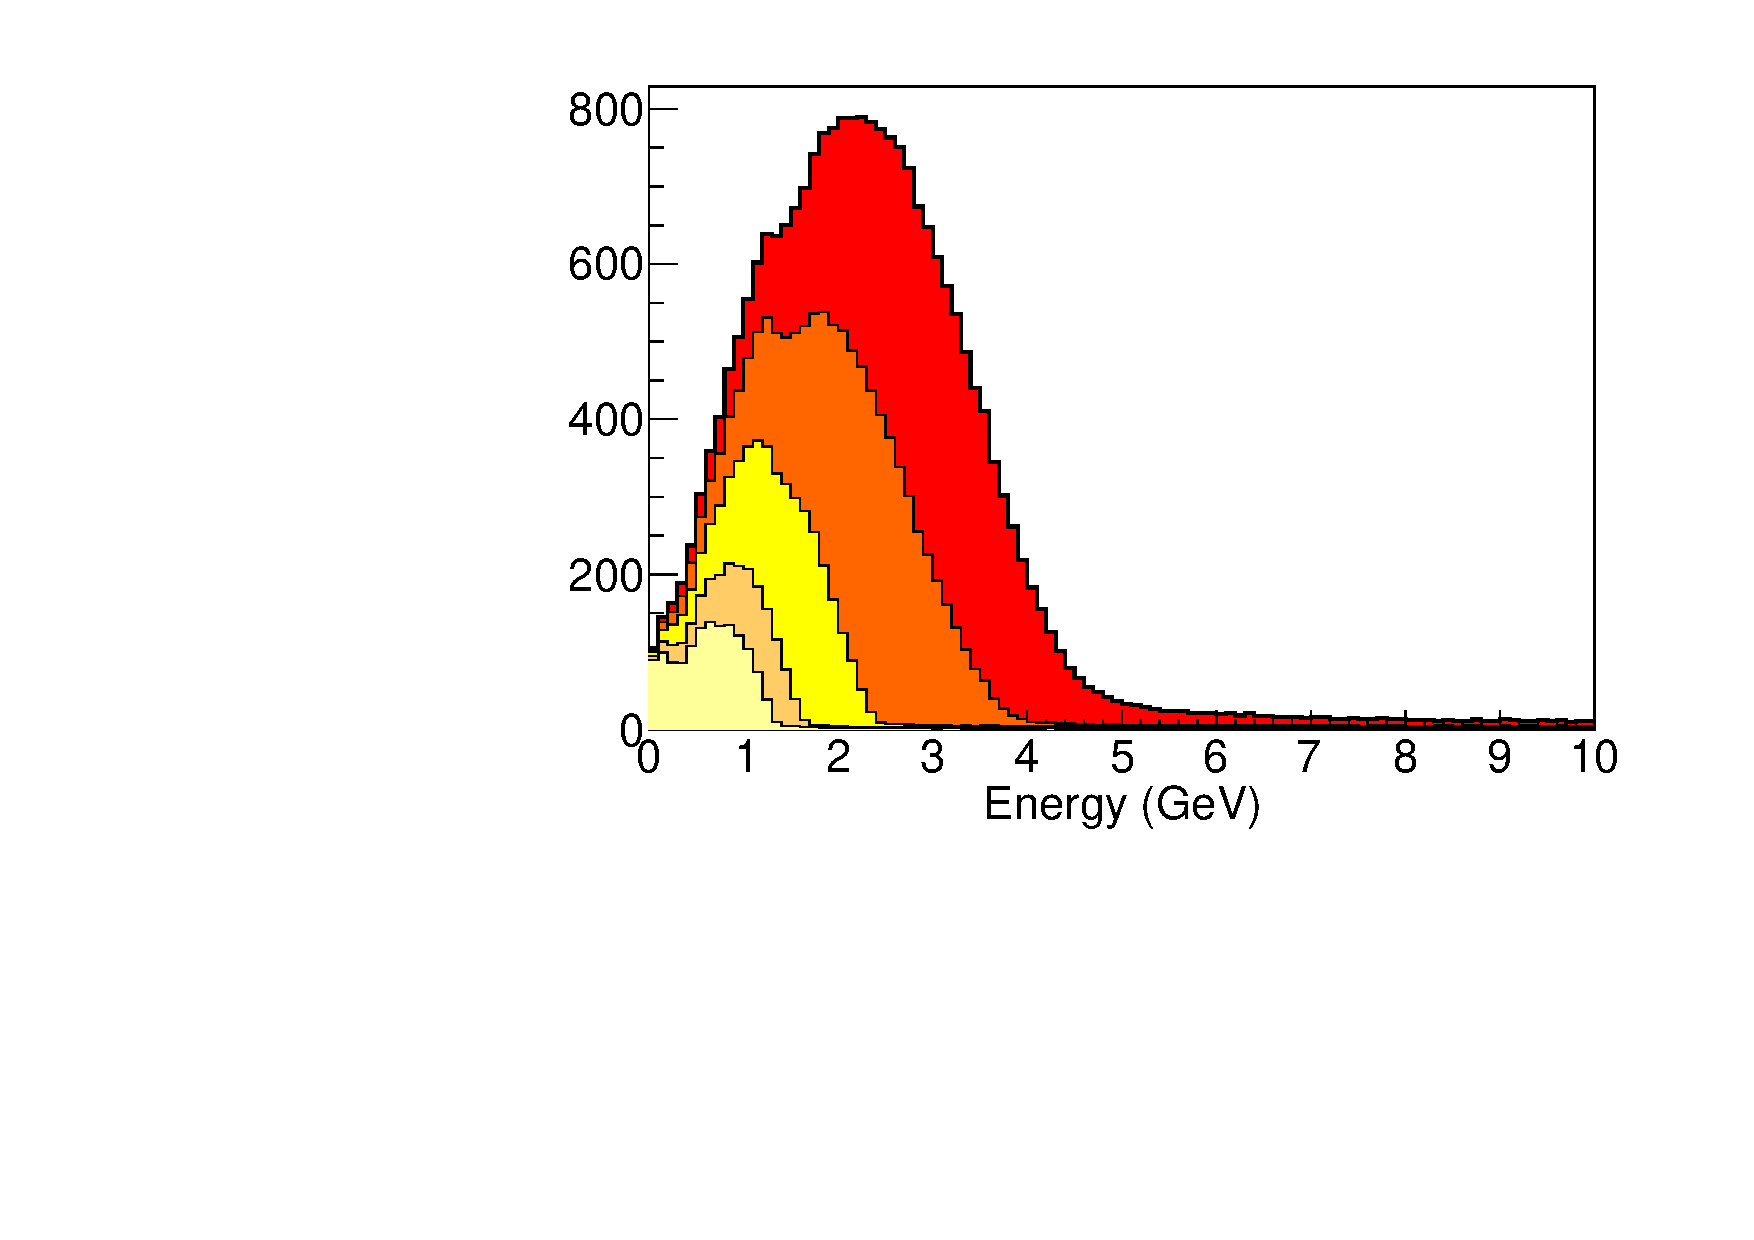
\includegraphics[width=0.49 \linewidth]{Figures/2018.10.10_LBNFtiming/DUNEbeam_truetimingB.pdf} &
			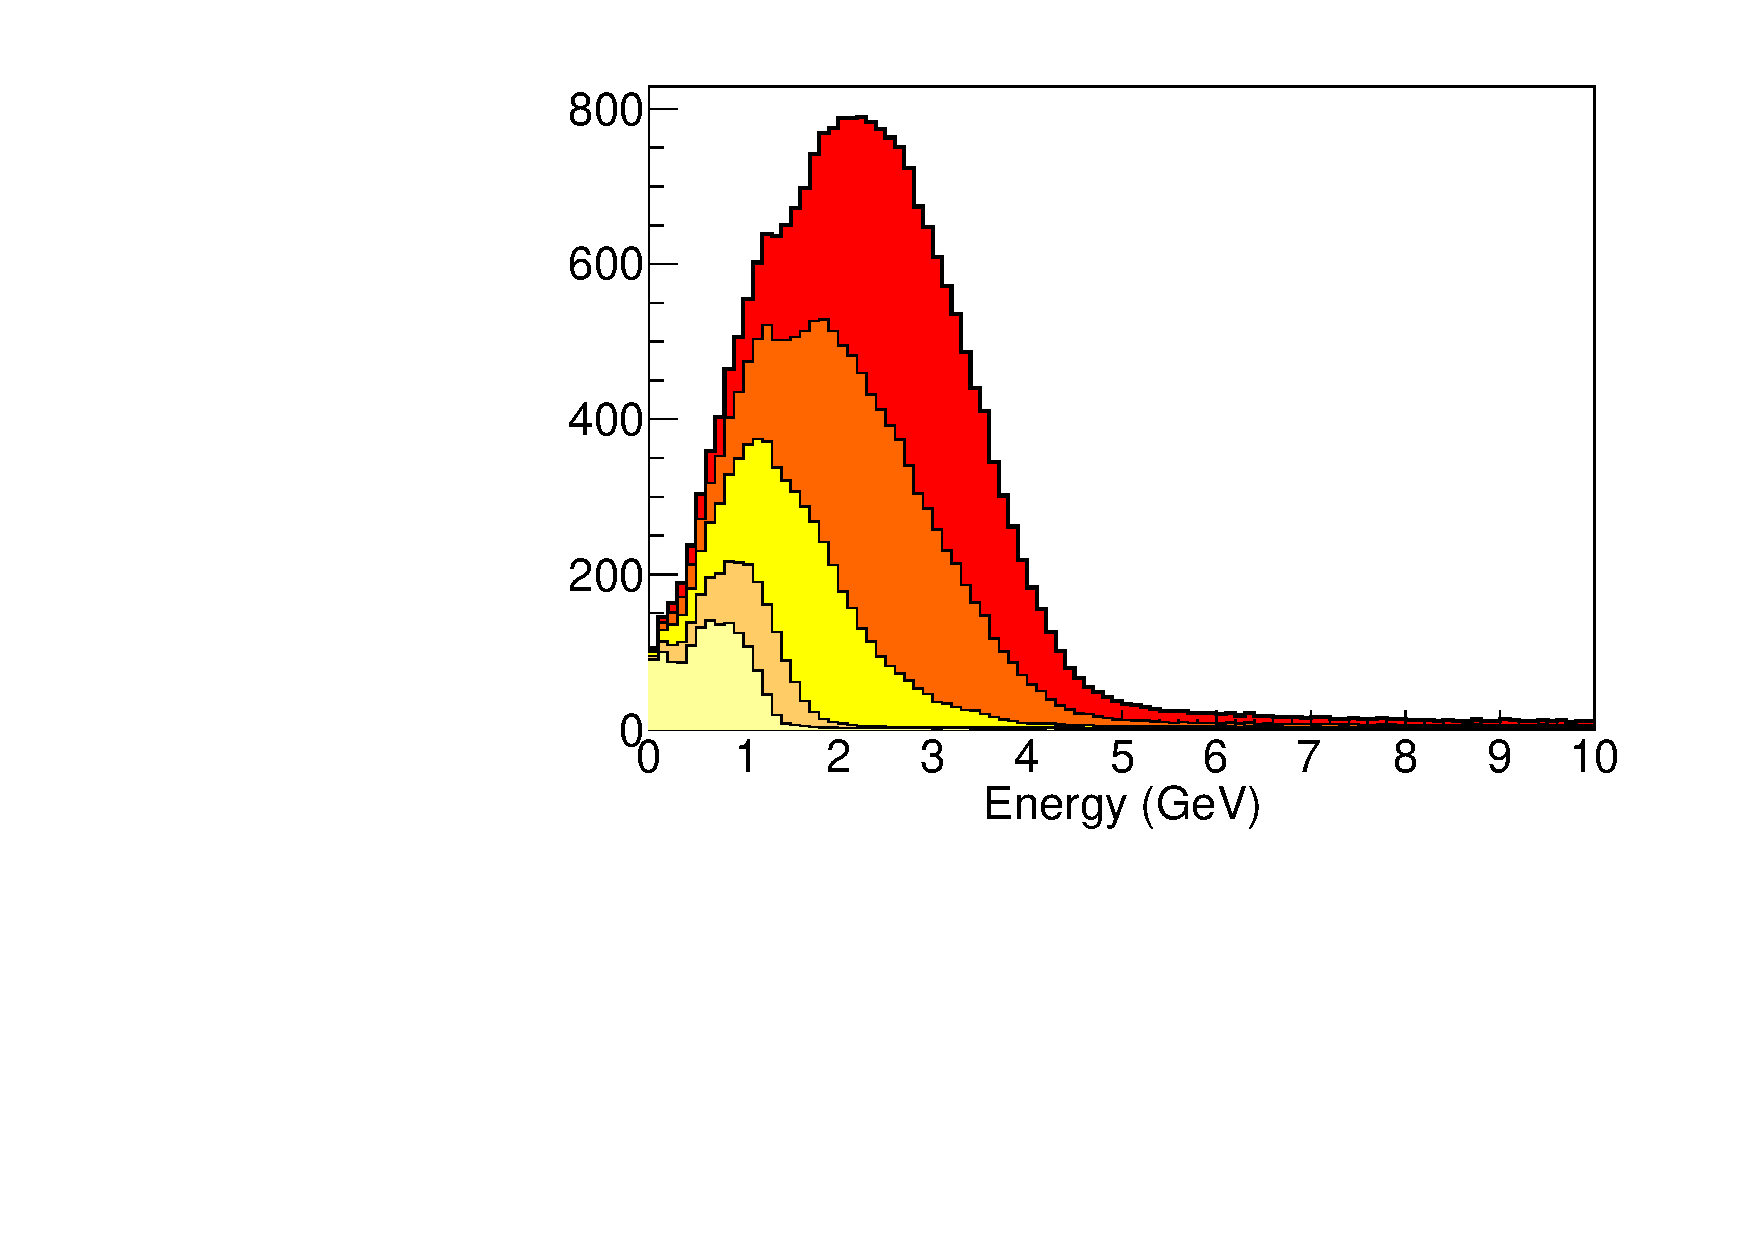
\includegraphics[width=0.49 \linewidth]{Figures/2018.10.10_LBNFtiming/DUNEbeam_100psecB.pdf} \\
           	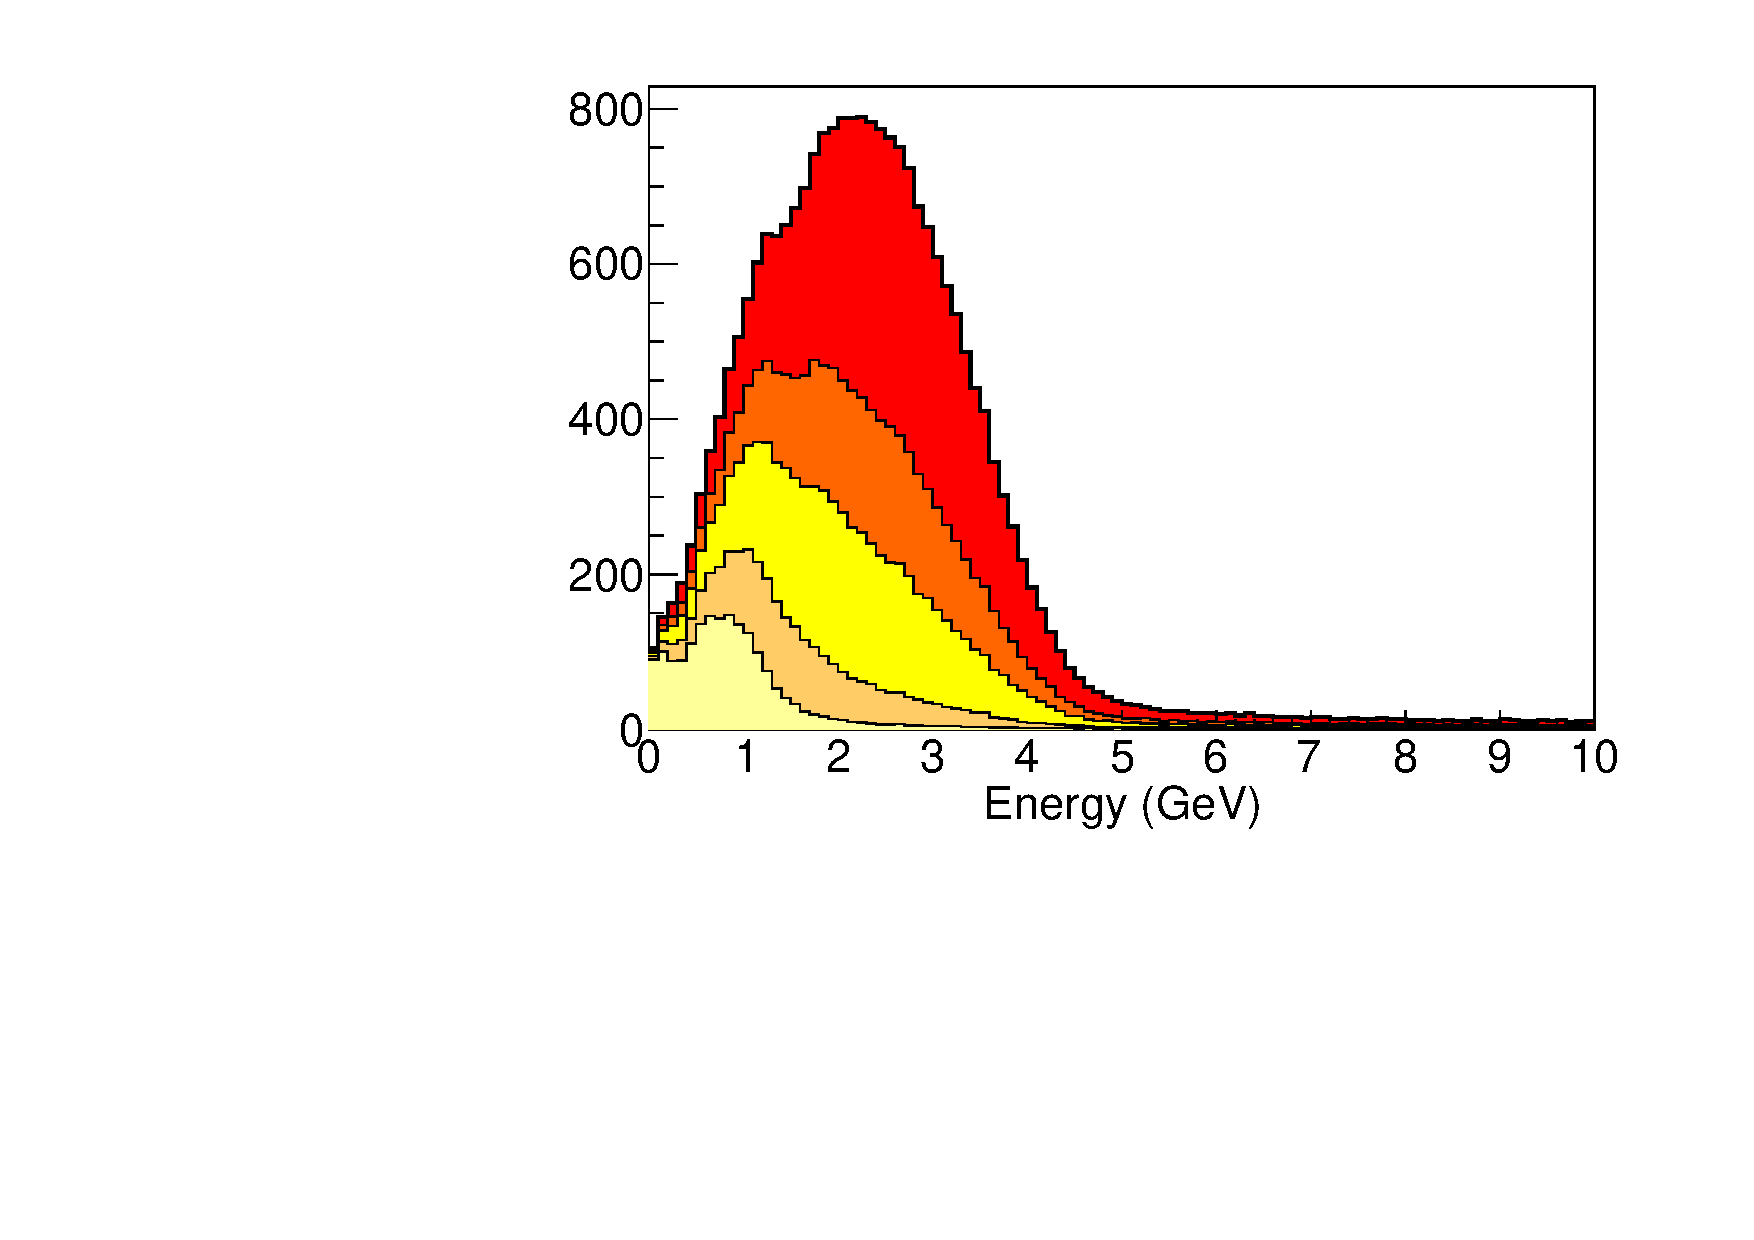
\includegraphics[width=0.49 \linewidth]{Figures/2018.10.10_LBNFtiming/DUNEbeam_250psecB.pdf} &
			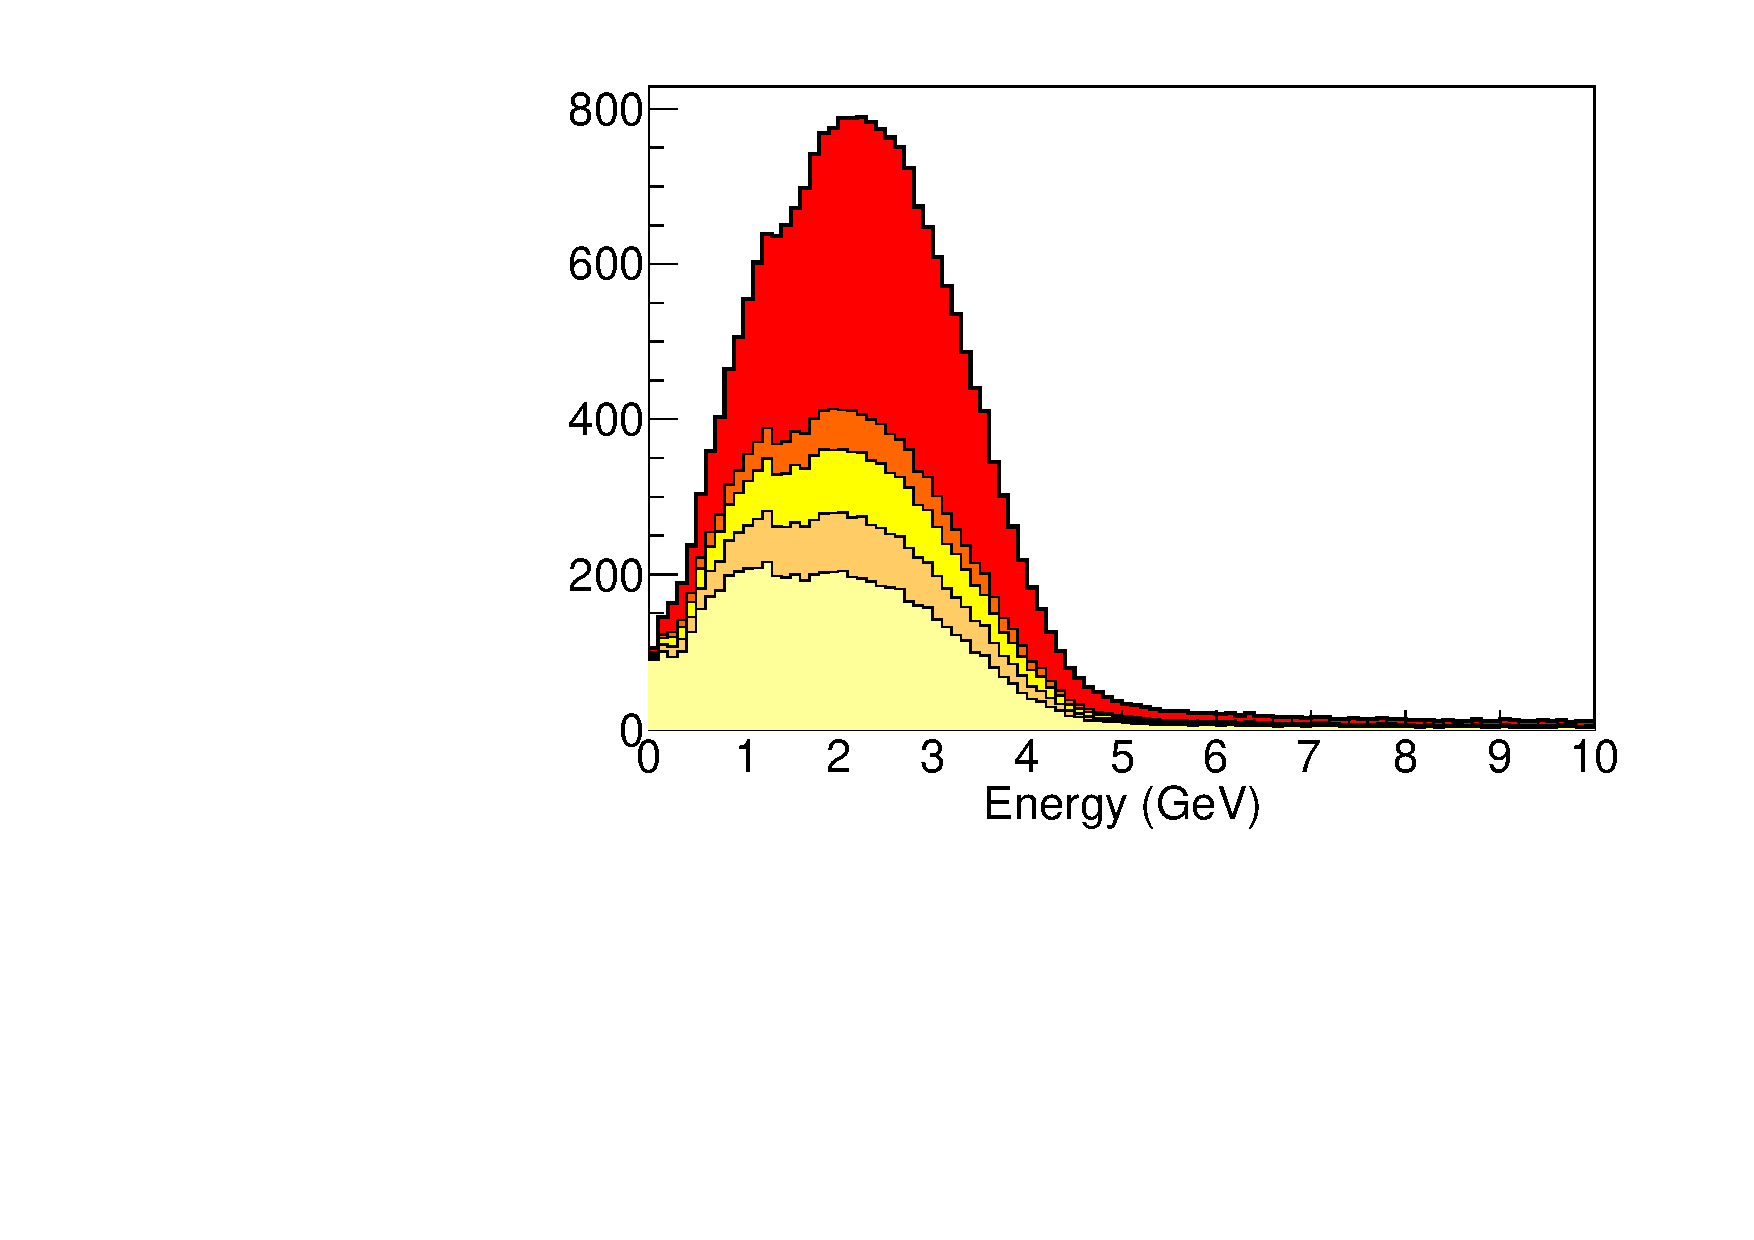
\includegraphics[width=0.49 \linewidth]{Figures/2018.10.10_LBNFtiming/DUNEbeam_900psecB.pdf}
			 \\			
			\end{tabular}
	\end{center}
	\caption{A series of panels showing the DUNE forward horn current flux (red), overlaid with the fluxes corresponding to increasingly later time-cuts on the bunch time, assuming no time spread of the protons on target: 250 psec after the start of the neutrino bunch (orange), 500 psec after (yellow), 750 psec (dark beige), 1 nsec (light beige). The UPPER LEFT panel corresponds to a case where all protons hit the target instantaneously. The UPPER RIGHT panel corresponds to a proton bunch with 100 psec width. The LOWER left panel corresponds to a 250 psec bunch width and the LOWER RIGHT corresponds to 900 psec.}
		\label{fig:anniedetector}
\end{figure}


\section{Superimposing a Fine Bunch Structure at 500 MHz: Concept and Feasibility}

Talking about how this could be done, how big a change it would be, how hard, etc

\section{Achieving 100 psec Relative Timing Resolution}

Jonathan Eisch - getting beam information, making fast triggers, etc

\section{Achieving 100 psec Vertex Resolution}


\section{Conclusion}

This is great.

%% The Appendices part is started with the command \appendix;
%% appendix sections are then done as normal sections
%% \appendix

%% \section{}
%% \label{}

%% References
%%
%% Following citation commands can be used in the body text:
%% Usage of \cite is as follows:
%%   \cite{key}          ==>>  [#]
%%   \cite[chap. 2]{key} ==>>  [#, chap. 2]
%%   \citet{key}         ==>>  Author [#]

%% References with bibTeX database:

\bibliographystyle{model1-num-names}
\bibliography{bibliography.bib}

%% Authors are advised to submit their bibtex database files. They are
%% requested to list a bibtex style file in the manuscript if they do
%% not want to use model1-num-names.bst.

%% References without bibTeX database:

% \begin{thebibliography}{00}

%% \bibitem must have the following form:
%%   \bibitem{key}...
%%

% \bibitem{}

% \end{thebibliography}


\end{document}

%%
%% End of file `elsarticle-template-1-num.tex'.